\documentclass[svgnames,tikz]{standalone}

\usetikzlibrary{decorations.pathmorphing,decorations.pathreplacing}

\begin{document}
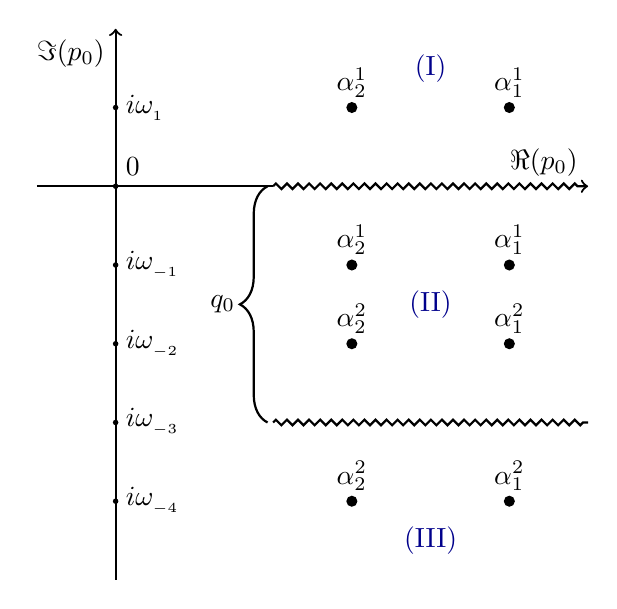
\begin{tikzpicture}[thick]

  \def\xrange{6} \def\yrange{4}
  % Axes
  \draw (-1,0) -- (2,0);
  \draw[->,decorate,decoration={zigzag,segment length=4,amplitude=1,post=lineto,post length=3}]
  (2,0) -- (\xrange,0) node[above left] {$\Re(p_0)$};
  \draw[decorate,decoration={zigzag,segment length=4,amplitude=1}] (2,-3) -- (\xrange,-3);
  \draw [->] (0,-\yrange-1) -- (0,2) node [below left=0.2] {$\Im(p_0)$};

  \draw[decorate,decoration={brace,amplitude=10pt,mirror},xshift=-2pt] (2,0) -- (2,-3) node [midway,left=8pt] {$q_0$};

  % Matsubara frequencies
  \foreach \n in {-\yrange,...,-1,1}{%
      \fill (0,\n) circle (1pt) node [right] {$i \omega_{_{\n}}$};}
  \fill (0,0) circle (1pt) node [above right] {0};

  % Poles
  \fill
  (3,1) circle (2pt) node[above] {$\alpha_2^1$}
  (5,1) circle (2pt) node[above] {$\alpha_1^1$}
  (3,-1) circle (2pt) node[above] {$\alpha_2^1$}
  (5,-1) circle (2pt) node[above] {$\alpha_1^1$}
  (3,-2) circle (2pt) node[above] {$\alpha_2^2$}
  (5,-2) circle (2pt) node[above] {$\alpha_1^2$}
  (3,-4) circle (2pt) node[above] {$\alpha_2^2$}
  (5,-4) circle (2pt) node[above] {$\alpha_1^2$};

  % Regions
  \node[DarkBlue] at (4,1.5) {(I)};
  \node[DarkBlue] at (4,-1.5) {(II)};
  \node[DarkBlue] at (4,-4.5) {(III)};

\end{tikzpicture}
\end{document}
